\documentclass[11pt]{article}
\usepackage{acl2012}
\usepackage{geometry}
\usepackage{latexsym}
\usepackage{amsmath}
\usepackage{multirow}
\usepackage{url}
%\usepackage[numbers]{natbib}
\usepackage{graphicx}
\usepackage{subcaption}
\usepackage{float}
\newgeometry{margin=2.85cm}
\DeclareMathOperator*{\argmax}{arg\,max}
\setlength\titlebox{3.8cm}    % Expanding the titlebox

\graphicspath{{../figures/}}

\title{{\small CS224W Final Project} \\ What is karma? Quantifying online influence and credibility}
\author{Thomas Dimson \\
  {\tt tdimson@cs.stanford.edu}
  \\\And
  Milind Ganjoo \\
  {\tt mganjoo@stanford.edu}
}
\date{}

\begin{document}
\maketitle

\newcommand{\citet}[1]{\cite{#1}}

\section{Introduction}
Many online communities explicitly publicize the concept of \textit{karma} or
\textit{reputation} for users, computed as a sum of positive votes by other members of
the community. These explicit measures are often seen as proxies for more
intangible notions such as \textit{influence} (the ability of a member to
persuade others) and \textit{credibility} (the trustworthiness of the user as an
member of the community). In this paper, we describe the range of network
characteristics, interactions, and temporal factors that affect the accumulation
of karma points. Using this, we build a model that predicts karma values.

While our model is evaluated on datasets that contain an explicit
measure of karma, we are particularly motivated by the ability of the
model to generalize to \textbf{private} communities. For example, our model can
be applied to e-mail interaction graphs to determine a ``karma'' score for members
of an organization. 

\section{Prior Work}

Most prior literature focuses on the abstract quality of \textit{influence}.
Both \citet{bakshy2011everyone} and \citet{cha2010measuring} define
influence as the ability to generate cascades on the Twitter graph. The authors
use local feature of users (e.g.\ number of followers, number of tweets,
retweets, mentions) in order to predict the ability for users to generate
cascades.

\citet{cha2010measuring} emphasizes the topic-specificity of influence -- they challenge
the notion that there is a common set of ``influentials'' who have
broad-reaching impact on online communities. Instead, they demonstrate that for
many topics, such as political events, there are special interest groups like
bloggers and politicians that see higher retweet and mention scores than the
generally popular Twitter users.

In a very recent paper, \citet{movshovitzanalysis} consider the reputation
scheme on StackOverflow (based on upvotes and accepted answers). They 
attempt to identify expert users based on their contribution
patterns and use high reputation users for validation. The authors tried many 
techniques to improve their classifier performance including PageRank and
an SVD decomposition of their interaction graphs. Notably, they find
that PageRank does not contribute significantly to their performance
and use user features such as number of answers, questions and question-answer 
rations in their final random forest model. They are
able to achieve an Area under the Curve of 81\% when classifying users
with reputations of more than 2400.

\section{Dataset}
In this paper, we will be focusing on two relatively large internet communities:
\textbf{Hacker News} and the \textbf{StackExchange} family of
websites. On Hacker News, users submit technology-related stories as
\textit{submissions} which other users use as an anchor to threaded discussions.
A user's \textit{karma} is computed as a sum of up-votes to their stories and
comments.  The StackExchange family of websites are question-and-answer sites
where a user will post a question and solicit answers from the community. A
user's \textit{reputation} is a weighted sum based on the number of their
questions and answers that are accepted, and whether their comments and posts
are voted as helpful by the community.

Gathering data for Hacker News came with many challenges: there is no published
dump of hacker news data, and no official API. Fortunately, the creator
of ThriftDB has created HNSearch\footnote{\url{https://www.hnsearch.com/}} as a technology
demo for his database. In addition to a public website, there is an unofficial API
supporting search queries. Although the API is limited to collecting 
only 100 recent items, we were able to circumvent this by constructing queries with limited
date ranges. Over the course of a week, we extracted JSON files for every comment,
submission and user on Hacker News by repeatedly querying the API\@. To our knowledge,
ours is the only complete dump of this data available on the internet.

Collecting data for the StackExchange family of websites was relatively easier.
An anonymized data dump of the entire series of websites is released every three
months\footnote{http://www.clearbits.net/creators/146-stack-exchange-data-dump}
in XML format. We wrote a Python script to parse the XML data and extract
relevant fields. Our initial emphasis is on \textbf{Super User}, which is a website where
enthusiasts and power users users ask questions about various aspects of
computer software and hardware. We chose this website because the data
is smaller in size since the website is new relative to Stack Overflow, the first
website in the StackExchange network. For the final report, however, we will
also include analysis on StackOverflow data.

After collecting the raw data for both datasets, we created an SQLite database
with normalized columns for all the fields. We also created an interaction graph
by collecting $(\text{replier}, \text{parent poster})$ edges and then caching
the graphs on disk as a NetworkX structure. A summary of our datasets is
available in Table~\ref{tab:graphstats}. As a final step, we divided each dataset 
into train, validation and test sets at
a 70\%/15\%/15\% split. Our milestone results are reported on our validation
set.

\begin{table*}[t]
\begin{center}
\begin{tabular}{| r | l l |}
\hline
& \textbf{Hacker News} & \textbf{Super User} \\
\hline
Users (Nodes) & 175091 & 190781 \\
Replies (Edges) & 2747966 & 266673 \\
Average Karma / Reputation & 131.8 & 83.1 \\
Largest SCC Fraction & 43\% & 3.8\% \\
Largest WCC Fraction & 63\% & 46\% \\
\hline
\end{tabular}
\end{center}
\caption{Graph statistics for our implied interaction graphs}
\label{tab:graphstats}
\end{table*}

\section{Model and Features}
Below we describe the karma and reputation distributions for both networks.
After establishing the nature of the data, we investigate the association 
between a number of features and karma/reputation. 

\subsection{Karma Distribution}
% Power law plots, etc.

\subsection{Karma Cliques and Preferential Attachment}
One model that seems intuitive is that high reputation users
tend to attach to other high reputation users, forming so-called
\textit{karma cliques}. We initially tested this hypothesis by
logarithmatically-bucketing karma/reputation and computing 
\citet{newman2003mixing}'s assortiativity over karma levels. This yields
relatively low assortiativity of $0.015$ and $0.040$ on Hacker News
and SuperUser respectively. As such, we see \textit{no evidence} of 
preferntial attachment on either network.

Beyond correlations, Figure~\ref{fig:karma_cliques}
shows a scatter plot of the average of neighboring karma. In both networks,
the mean average neighboring karma remains relatively constant at all
karma levels, although the variance shrinks as karma increases.
Super User's plot is dramatically different than Hacker News. While there is
no discernable pattern based on the anchor node's karma, there is a noticable
clustering between looking at inbound reputation and outbound reputation. We see
that the inbound reputation (people answering this post) tends to be much higher
than the outbound karma (the questioner's karma). This suggests two distinct
roles on SuperUser: the questioners and the answers. Hacker News does not
appear to have this distinction.

\begin{figure*}[t]
\centering
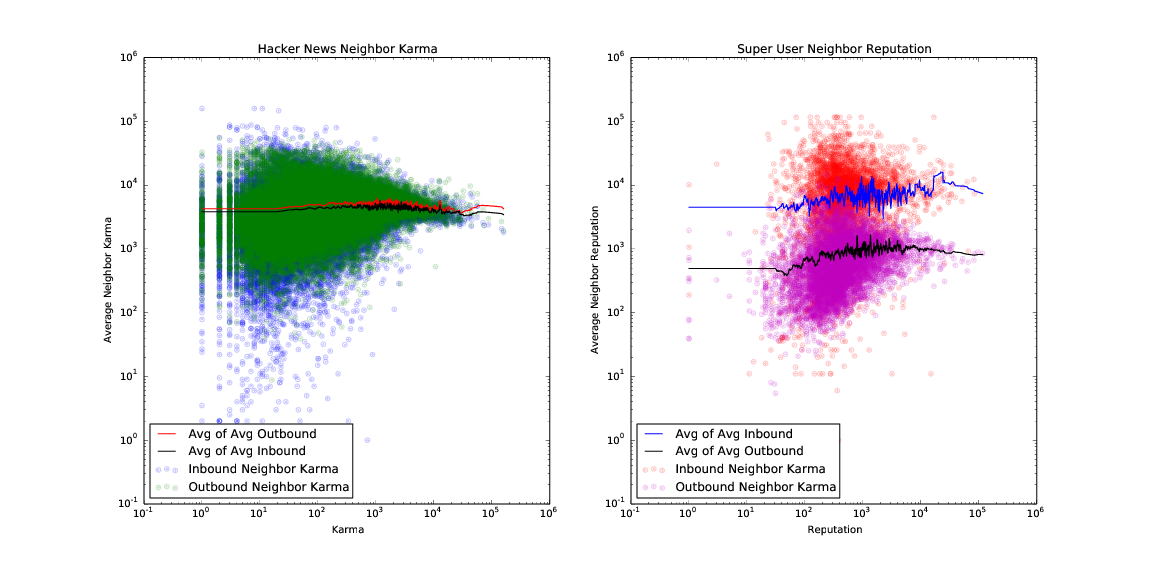
\includegraphics[width=\linewidth]{karma_cliques}
\caption{Scatter plot of average neighbor karma against the anchor node's karma. 
The lines represent the mean average neighbor karma at a given karma level.
Neighbor karma variance appears to shrink with larger anchor karma values.}
\label{fig:karma_cliques}
\end{figure*}

\begin{figure*}[t]
\centering
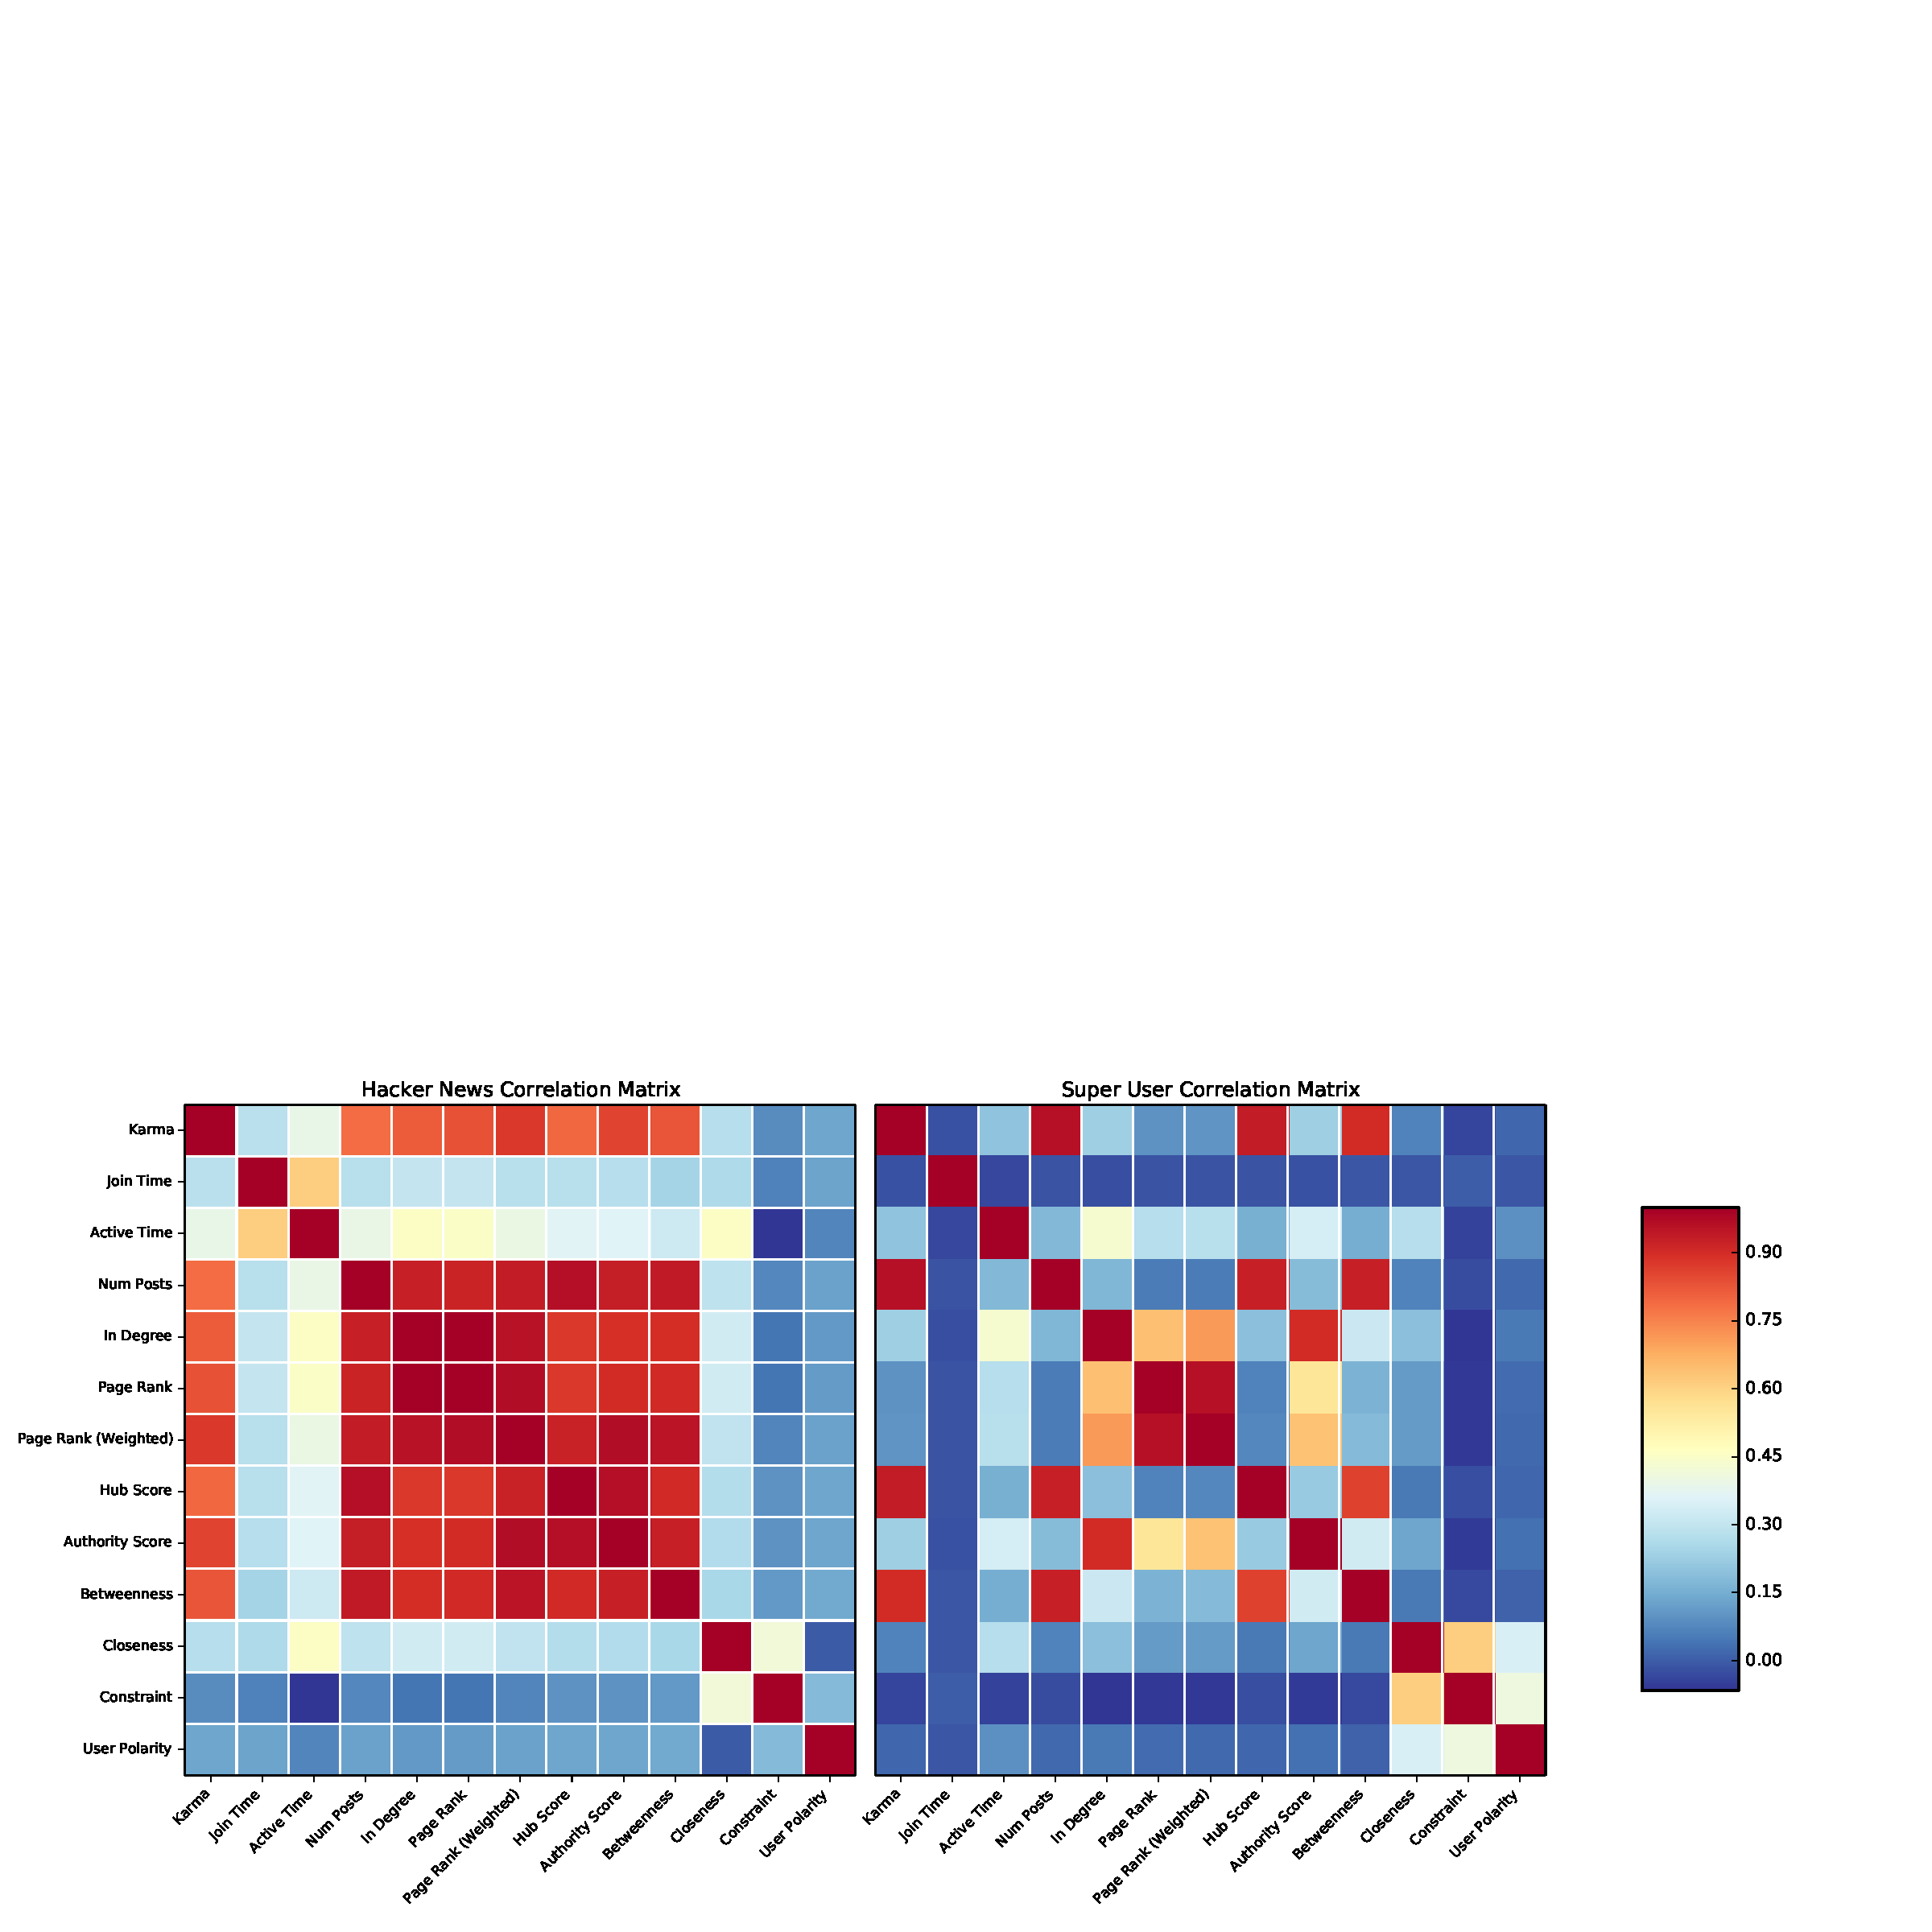
\includegraphics[width=\linewidth]{correlation}
\caption{Pearson's corrrelation coefficient matrix for some of our features.
Notice the dramatic difference in the types correlations when switching
between Hacker News and SuperUser.}
\label{fig:correlation}
\end{figure*}

\subsection{Node Features}
% Time spent on the site, etc.

\subsection{Graph Features}

% PageRank, Constraint, HITS, etc. This should be most of it

\subsection{Textual Features}
% LDA, Sentiment, etc.


\section{Evaluation}
%Summary table would go here

\subsection{High-karma Prediction}
% ROC curves

\subsection{Karma regression}
% Divided into section

\section{Conclusion}

\bibliography{report}{} \bibliographystyle{acl2012}

\end{document}
